\chapter{Polar Codes in 5G} \label{polarCodes}
Polar codes are a class of capacity-achieving codes introduced by Ar\i kan in 2009 \cite{Arikan}. $ 5^{th} $ generation wireless systems (5G) has adopted polar codes as the channel coding candidates for uplink and downlink control information for the enhanced mobile broadband (eMBB) \cite{3gpp.38.212}. This chapter explains the details about different types of 5G physical channels which use polar codes for channel coding, purpose of these physical channels and used modulation formats. This chapter also presents the generic encoding FEC chain of the polar codes and explains the details about FEC chain parameters such as adopted polar code block-length sizes, Cyclic Redundancy Check (CRC) type, size et cetera.

Generic polar FEC chain is shown in Figure \ref{fig:Generic5gtx_fec_chain}. This FEC chain is configured with the parameters of a particular physical channel as specified in \cite{3gpp.38.212} and \cite{3gpp.38.211}.

\begin{figure}[!h]
	\centering
	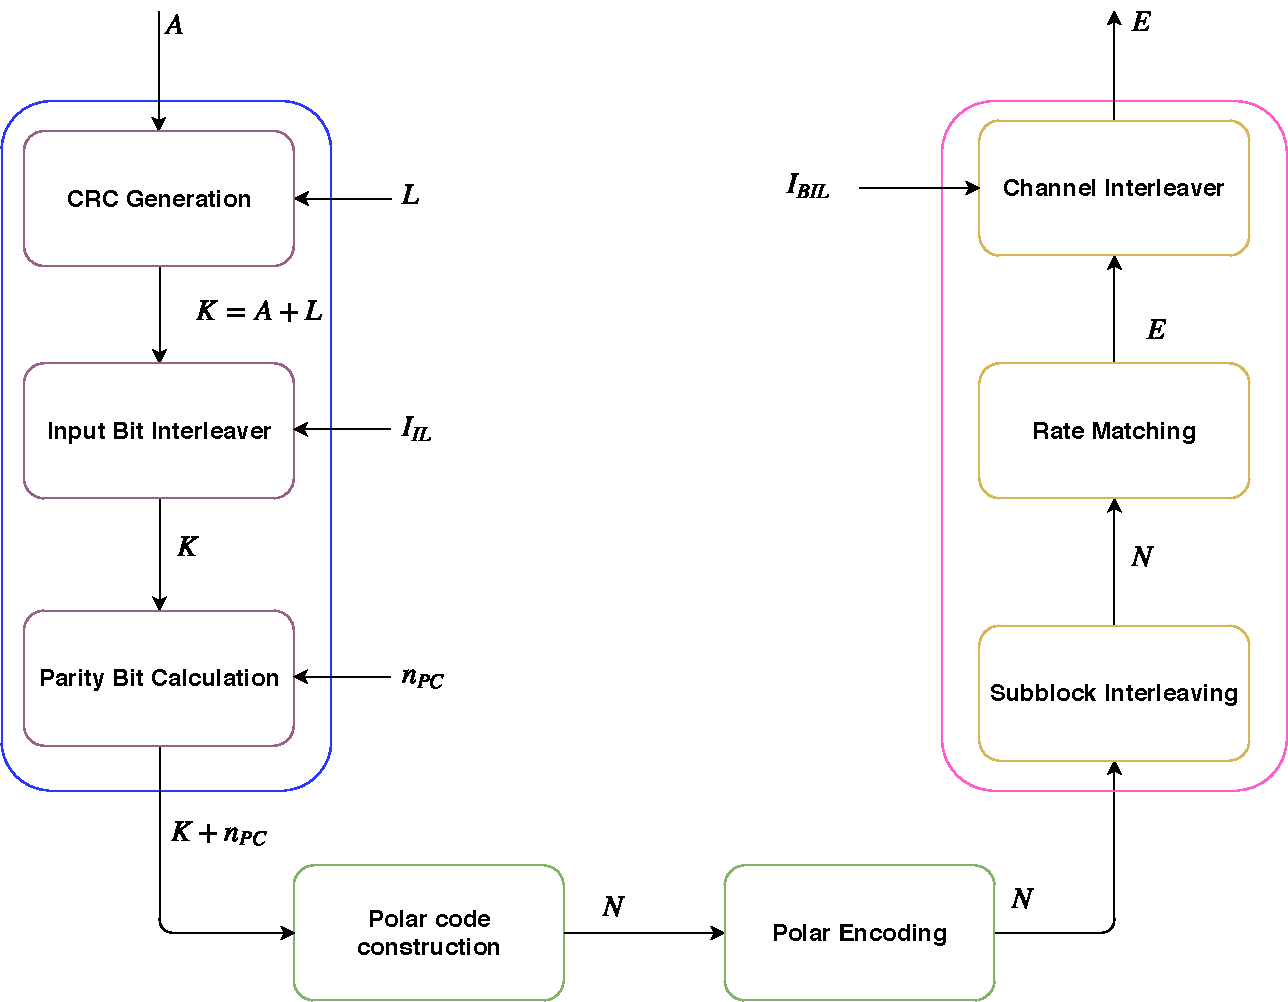
\includegraphics[width=0.7\textwidth]{./figures/Generic5GFECchain.pdf}
	\caption{Generic Encoding FEC of 5G}
	\label{fig:Generic5gtx_fec_chain}
\end{figure}

The polar FEC chain, receives $A$ information bits from the upper layer. These bits need to be transmitted through a code of length $E$ bits. Size of $A$ depends on the physical channel and size of uplink or downlink control information. Value of $ E $ depends on the scheduling and resource allocation parameters and it is configured from higher layers. After receiving $A$ information bits, a $L$-bit CRC is attached to the information bits resulting in $K = A + L$ bits. The  value of $L$ is determined based on the physical channel, size of $A$ and $E$. After attaching CRC bits, $K$ bits are interleaved by input bits interleaver. The input bits interleaver is configured with the parameter $I_{IL}$. $I_{IL}$ can take either 0 or 1. This module is enabled when $I_{IL} = 1$ otherwise input bits interleaver is disabled. Next component in the FEC chain is Parity Check (PC) bits calculation. Number of PC bits are configured with the parameter $n_{PC}$. $n_{PC}$ value is selected based on the physical channel, size of $A$ and $E$. Another parameter of PC component is $n_{pc}^{wm}$ which indicates how many parity bits need to be placed in the rows of minimum hamming weight in the polar code generator matrix \cite{3gpp.38.212}. After parity bits calculation, the polar code construction component identifies  $K + n_{PC}$ reliable indices for placing $A+L$ bits and $n_{PC}$ positions for parity bits. The parameter $N = 2^n$ is the block-length of polar code. Value of $n$ is calculated based on the values of $E$, $K$ and $n_{max}$. where $n_{max}$ is configured based the physical channel. In 5G polar FEC chain, five different block-lengths are supported as given by $\mathcal{N} = {32,64,128,256,512,1024}$. The encoded bits go through sub-block interleaving and rate matching to obtain $E$ bits from $N$ bit codeword. Next configurable parameter is $I_{BIL}$, it configures the channel interleaver. It can take either 0 or 1. $I_{BIL} = 1$ enables channel interleaver otherwise it is disabled. Details of the different physical channels and their FEC chain parameters are presented in the following sections.

\section{5G Physical Channels}
This section presents details of the 5G physical channels which use polar codes. The 5G standard adopted polar codes for uplink and downlink control channels. Uplink control channels carry information about channel quality indicators, acknowledgments et cetera. In downlink control channels carry resource allocation information, uplink power control instructions and the information required for the user equipment (UE) to access the network. Following sections explain each of these uplink and downlink control channels and their polar FEC chain parameters.

\subsection{Physical Broadcast Channel (PBCH)}
In downlink, polar coding is applied to PBCH which carries the essential information required for the UE to access the network. PBCH carries network information such as system bandwidth, current system frame sequence et cetera. The polar FEC chain parameters of PBCH are fixed. In other words, payload size ($A$) of PBCH is always 56 bits. Other fixed parameters of PBCH are $E = 846$, $L = 24$, $n_{max} = 9$, $I_{IL} = 1$, $I_{BIL} = 0$, and $n_{PC} = n_{pc}^{wm} = 0$. Modulation format used for PBCH is always QPSK. PBCH is explained in more detail in \cite{3gpp.38.212}.

\subsection{Physical Downlink Control Channel (PDCCH)}
The PDCCH is an another downlink control channel which uses polar codes. Resources requested by the UE are assigned by the base station. This resource allocation information is transmitted via PDCCH channel. PDCCH also carries information related to uplink power control, downlink resource grant and system paging information \cite{3gpp.38.211}. The PDCCH contains a message called Downlink Control Information (DCI) which carries all the control information of UE. Payload size of PDCCH is not fixed. It varies based on the format of DCI, As a consequence, values of $A, N$ and $E$ vary. Type of DCI is configured from higher layer. Except $A, N$ and $E$, other parameters of the PDCCH polar FEC chain are same as PBCH. Complete details about different DCI formats in PDCCH are presented in Section 7.3 of \cite{3gpp.38.212}.

\subsection{Physical Uplink Control Channel (PUCCH)}
In uplink, PUCCH contains Uplink Control Information (UCI) similar to DCI in the downlink. UCI carries channel state information, acknowledgments, scheduling request et cetera. The payload size of PUCCH varies based on the PUCCH formats \cite{3gpp.38.211}. PUCCH uses different channel coding techniques depending on payload size. When payload size $A \geq 12$ polar codes are used. PUCCH polar FEC chain parameters also vary depending on the values of $A$ and $E$. \newline

$\bullet$ There are three different cases for PUCCH polar FEC chain parameters based on the values of $A$ and $E$ as presented below. \newline

$\bullet$ \emph{Case 1. $A \geq 20 $} \newline
\hspace*{2em}$L = 11$, $n_{max} = 10$, $I_{IL} = 0$, $I_{BIL} = 1$, and $n_{PC} = n_{pc}^{wm} = 0$. \newline
	 
$\bullet$ \emph{Case 2. $12 \leq A \leq 19 $ and $E-A \leq 175 $} \newline
\hspace*{2em}$L = 6$, $n_{max} = 10$, $I_{IL} = 0$, $I_{BIL} = 1$, and $n_{PC} = 3 $, $n_{pc}^{wm} = 0$. \newline

$\bullet$ \emph{Case 3. $12 \leq A \leq 19 $ and $E-A \geq 175 $} \newline
\hspace*{2em}$L = 6$, $n_{max} = 10$, $I_{IL} = 0$, $I_{BIL} = 1$, and $n_{PC} = 3 $, $n_{pc}^{wm} = 1$. \newline

PUCCH uses $\pi/2$-BPSK or QPSK depending on the PUCCH format \cite{3gpp.38.211}.

\subsection{Physical Uplink Shared Channel (PUSCH)}
PUSCH is an another uplink channel which transmits UCI. In PUSCH, LDPC codes are used for encoding user data and polar codes for control information. The UE transmits UCI in PUCCH, if UE is not transmitting any user data to the base station. When UE is transmitting user data through PUSCH, UCI is also transmitted with PUSCH using the same modulation parameters. In other words, if PUSCH is using 64-QAM then same modulation technique is applied to UCI. Allowed modulation formats for PUSCH are QPSK, 16-QAM, 64-QAM and 256-QAM as presented in Section 6.3.1.2 of \cite{3gpp.38.211}. \newline

The parameters of polar FEC chain for different physical channels of 5G are summarized in the Table \ref{tab:FecChainParameters}.

\begin{table}[!h]
	\caption{Channel parameters \cite{DesignOfPolarCodes5G}}
	\label{tab:FecChainParameters}
	\begin{tabular}{c|c|c|c|c|}
		\cline{2-5}
		\multirow{3}{*}{}               & \multicolumn{3}{c|}{PUCCH/PUSCH}                                                         & \multirow{2}{*}{PDCCH/PBCH} \\ \cline{2-4}
		& \multirow{2}{*}{$A\geq20$} & \multicolumn{2}{c|}{$12\leq A\leq 19$} &                             \\ \cline{3-5} 
		&                                     & $E-A \leq 175$     & $E-A \geq 175$    &                             \\ \hline
		\multicolumn{1}{|c|}{$n_{max}$}      & \multicolumn{3}{c|}{10}                                                                  & 9                           \\ \hline
		\multicolumn{1}{|c|}{$I_{IL}$}       & \multicolumn{3}{c|}{0}                                                                   & 1                           \\ \hline
		\multicolumn{1}{|c|}{$I_{BIL}$}      & \multicolumn{3}{c|}{1}                                                                   & 0                           \\ \hline
		\multicolumn{1}{|c|}{$L$}         & 11                                  & \multicolumn{2}{c|}{6}                             & 24                          \\ \hline
		\multicolumn{1}{|c|}{$n_{PC}$}     & 0                                   & \multicolumn{2}{c|}{3}                             & 0                           \\ \hline
		\multicolumn{1}{|c|}{$n_{pc}^{wm}$} & 0                                   & 0                       & 1                        & 0                           \\ \hline
	\end{tabular}
\end{table}